\section{Algoritmos de generación de señalamiento}
    \label{sec:generacion}
    
    En esta Sección se abordará la generación automática de señalamiento que realiza el RNA para cada uno de los elementos ferroviarios básicos y se mostrará como los principios de señalamiento (ver Sección \ref{sec:principios}) se cumplen para cada uno de ellos de forma individual. Se asumirá para el análisis de la red ferroviaria que todas las vías son bidireccionales y que los elementos ferroviarios deben ser protegidos en todas las direcciones. De esta forma, siempre se tendrá un análisis completo de la red ferroviaria, contemplando todos los posibles usos de la red que el operador pueda darle.
    
    Tal como se explico en la Sección \ref{sec:validacion}, al ser el modelo ferroviario de grafos un sistema lineal, podemos definir un principio de superposición de señales. Las señales generadas para un sistema con elementos ferroviarios A y B serán la superposición de las señales generadas para proteger al elemento A y las señales generadas para proteger al elemento B. No obstante, puede darse el caso de que una señal que originalmente protegía al elemento A también cumpla la función de proteger a B, por lo cual existe un solapamiento de señales. Por lo tanto, el señalamiento final tendrá menos señales que la suma de los señalamientos originales. Podemos generalizar esta conclusión en la siguiente fórmula:

    \[ \text{señales(a,b,\dots,z)} = \sum_{\text{elemento}=a}^{z} \text{señales(elemento)} - \displaystyle\bigcap_{\text{elemento}=a}^{z} \text{señales(elemento,elemento+1)} \]
    \[ \text{señales(a,b,\dots,z)} \leq \sum_{\text{elemento}=a}^{z} \text{señales(elemento)} \]

    Es decir, el señalamiento total siempre será menor a la suma del señalamiento generado para cada uno de los elementos ferroviarios, salvo que no existan señales solapadas. Para obtener el señalamiento final, el RNA debe no solo generar el señalamiento para cada elemento y combinarlo, sino también detectar solapamientos, inconsistencias o señales contradictorias que puedan comprometer la seguridad de la red y eliminarlas. La eliminación de señales deberá realizarse con ciertos criterios, para no disminuir el nivel de seguridad de la red ferroviaria. El proceso de simplificación del señalamiento se abordará en detalle en la Sección \ref{sec:simplificacion}.

    \subsection{Señalización en fin de vía y transiciones}
    
	\label{sec:sig_border}
    
    % Autoridad > derecho limitado a una porcion
    % Claridad > autoridad no ambigua
    % Anticipacion > avisar con antelacion
    % Granularidad > rutas cortas y funcionales
    % Terminalidad > avisar fin de via
    % Infraestructura > avisar de infraestructura
    % No bloqueo > circulacion fluida

    Tal como se definió en la Sección \ref{sec:bufferstop}, las redes ferroviarias presentan tanto fines de vía absolutos (modelados en railML por la clase \textit{bufferStop}) como fines de vía relativos (modelados en railML por la clase \textit{lineBorder}). El RNA detecta estos elementos y generará el señalamiento correspondiente en base a los principios de señalamiento expuestos en la Sección \ref{sec:principios}.

    En el caso de las transiciones para fines de vía relativos, por el principio de infraestructura ($P_6$), es necesario que existan señales que indiquen que la formación pueda circular por la transición de una región ferroviaria a otra. Esta señal debe otorgar autoridad a la formación de forma unívoca, por el principio de claridad ($P_2$). Adicionalmente, esa señal debe situarse con suficiente antelación a la transición, por el principio de anticipación ($P_3$). Aplicando el principio de no bloqueo ($P_7$) regulamos la circulación entre dos regiones ferroviarias para que puedan circular sin demoras ni atascos. Finalmente, el principio de granularidad ($P_4$) y autoridad ($P_1$) nos pide que el derecho de uso de la infraestructura debe ser acotado, pero funcional. Es decir, la autoridad debe aplicarse en una sección con un mínimo de largo como para que tenga sentido. 

    En el Algoritmo \ref{alg:lineBorder} aplicamos todos estos principios al solicitar que la sección donde colocamos la señal tenga un parámetro de largo mínimo. Además, al ser una transición, las señales colocadas son todas de partida, para transitar de una región a la otra, de ser permitido, o detener la formación en la frontera entre ambas regiones, de encontrarse saturada la próxima región.
    
    \begin{algorithm}[H]
        \caption{Algoritmo de generación de señalamiento para Line borders.}\label{alg:lineBorder}
        \DontPrintSemicolon
        %\SetAlgoLined
        \SetNoFillComment
        \LinesNotNumbered 
        \For { netElement WITH LineBorder }
        {
            \If { netElement.Length $>$ FIXED\_LENGTH }
            {
                \If { NOT EXIST next netElement }
                {
                    [Signals] $\gets$ ADD departure signal $\gg\gg$\;
                }
                \If { NOT EXIST prev netElement }
                {
                    [Signals] $\gets$ ADD departure signal $\ll\ll$\;
                }
            }
        }
        \KwResult{[Signals]} 
    \end{algorithm}

    En el caso de los \textit{buffer stops}, por el principio de terminalidad ($P_5$) es necesaria una señal que indique a las formaciones que deben detenerse antes de llegar al final de la vía. Además, es necesaria una señal de partida en sentido contrario para que las formaciones reanuden su marcha en el otro sentido. Esto fue implementado en el Algoritmo \ref{alg:bufferStop}. La restricción de tamaño fue removida porque el final de vía y la formación deben ser protegidos sin importar el largo de la sección.
    
    \begin{algorithm}[H]
        \caption{Algoritmo de generación de señalamiento para Buffer stops.}\label{alg:bufferStop}
        \DontPrintSemicolon
        %\SetAlgoLined
        \SetNoFillComment
        \LinesNotNumbered 
        \For { netElement WITH BufferStops }
        {
            \If { NOT EXIST next netElement }
            {
                [Signals] $\gets$ ADD stop signal $\gg\gg$\;
                [Signals] $\gets$ ADD departure signal $\ll\ll$\;
            }
            \If { NOT EXIST prev netElement }
            {
                [Signals] $\gets$ ADD stop signal $\ll\ll$\;
                [Signals] $\gets$ ADD departure signal $\gg\gg$\;
            }
        }
        \KwResult{[Signals]} 
    \end{algorithm}
    
    Aplicando el Algoritmo \ref{alg:lineBorder} y el Algoritmo \ref{alg:bufferStop} a dos vías paralelas con finales de vías relativos (vía superior) y absolutos (vía inferior) obtenemos un señalamiento como el que se visualiza en la Figura \ref{fig:signal_border}.
    
    \begin{figure}[H]
        \centering
        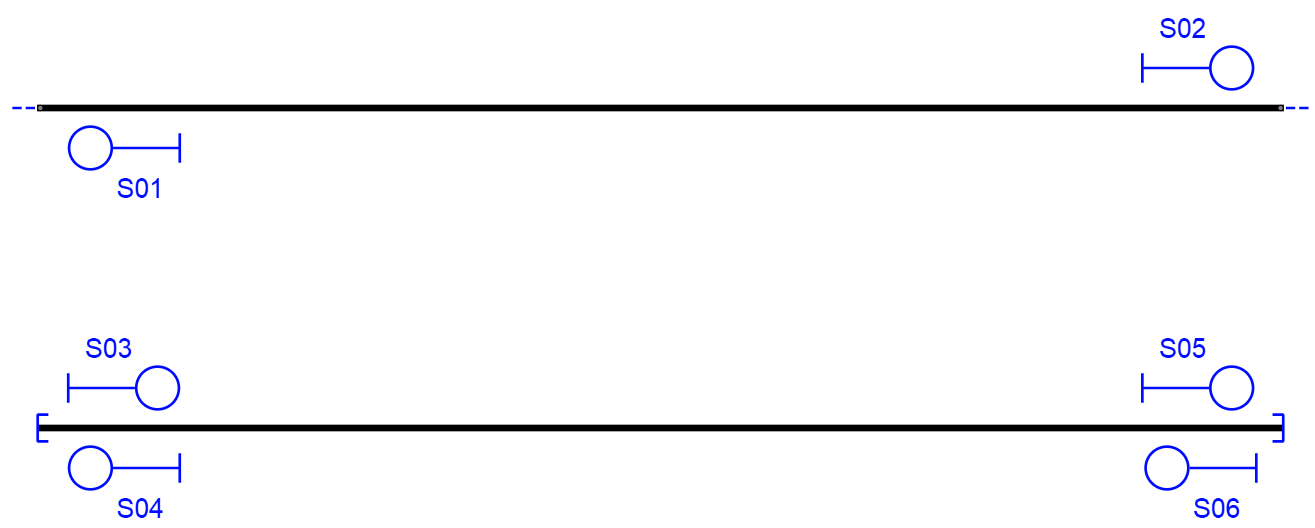
\includegraphics[width=1\textwidth]{Figuras/limites.PNG}
        \centering\caption{Señalamiento generado para finales de vía relativos y absolutos.}
        \label{fig:signal_border}
    \end{figure}
    
    El RNA detecta los \textit{line borders} en la vía superior y aplica el Algoritmo \ref{alg:lineBorder}, generando las señales de partida S01 para las formaciones que se mueven de derecha a izquierda y la señal de partida S02 para las formaciones que se mueven de izquierda a derecha, saliendo de la región mostrada en la Figura \ref{fig:signal_border}. Además, al detectar los \textit{buffer stops} en la vía inferior, el RNA aplica el Algoritmo \ref{alg:bufferStop}, generando cuatro nuevas señales. Las señales S04 y S05 son señales de parada para indicar a las formaciones que deben detenerse antes de colisionar con el final de la vía al transitar de derecha a izquierda o viceversa, respectivamente. Las señales S03 y S06 permiten a las formaciones reanudar su marcha en sentido contrario al que venían circulando, retomando su lugar en la red ferroviaria.
    \subsection{Detectores}

\lipsum[1]

\begin{algorithm}[hbt!]
            \caption{Train detection elements algorithm}\label{alg:RJ}
            \DontPrintSemicolon
            %\SetAlgoLined
            \SetNoFillComment
            \LinesNotNumbered 
            \For { netElement WITH AxleCounters or RailJoints }
            {
                Track.Length = Length ( between RailJoints )\;
                \If { Track.Length $>$ FIXED\_LENGTH }
                {
                    [Signals] $\gets$ ADD circulation signal $>>>$\;
                    [Signals] $\gets$ ADD circulation signal $<<<$\;
                }
            }
            \KwResult{[Signals]} 
        \end{algorithm} 
    \subsection{Plataformas ferroviarias}

    % Autoridad > derecho limitado a una porcion
    % Claridad > autoridad no ambigua
    % Anticipacion > avisar con antelacion
    % Granularidad > rutas cortas y funcionales
    % Terminalidad > avisar fin de via
    % Infraestructura > avisar de infraestructura
    % No bloqueo > circulacion fluida

    En la Sección \ref{sec:platform} definimos la clase platform que modela a las plataformas ferroviarias. Las plataformas ferroviarias son un punto del recorrido donde las formaciones pueden detenerse, algunas veces de forma opcional dependiendo el itinerario, para que los pasajeros desciendan y nuevos pasajeros puedan ascender. Claramente existe una limitación de autoridad, las formaciones necesitan un nuevo permiso para continuar circulando una vez alcanzada la plataforma. Permiso que será otorgado o negado según el estado del sistema a continuación del recorrido. Las plataformas ferroviarias suelen encontrarse en zonas pobladas, cerca de otras infraestructuras, zonas comerciales o residenciales, por lo que avisar con antelación al maquinista que debe disminuir la marcha y/o detenerse es esencial.

    Además, es posible que las formaciones convivan con otras formaciones que también hacen uso de la estación, por lo que las señales deben ser unívocas y claras. Algunas estaciones pueden contener fines de vías o ramificaciones hacia talleres u otros ramales, por lo que también se aplica el principio de terminalidad ($P_5$) y granuralidad ($P_4$). Finalmente, es importante el mantener una circulación fluida de las formaciones, de modo de no retrasar el itinerario de las formaciones que vienen detrás, por lo que se deberá aplicar el principio de no bloqueo ($P_7$).

    En el Algoritmo \ref{alg:PTF} definimos a la señal de partida como la única señal necesaria para operar una plataforma, asumiendo que la señal de ingreso de la misma será dada por otra instancia previa. De no existir otro elemento cercano por el cual se genere una señal, se puede asumir que la distancia a la plataforma es muy larga y, por lo tanto, se aplicaría el Algoritmo \ref{alg:RJ}, protegiendo a la plataforma. En el caso de que la vía sea bidireccional se añadiran señales de partida para ambos sentidos.

    \begin{algorithm}[hbt!]
        \caption{Algoritmo de generación de señalamiento para platforms.}\label{alg:PTF}
        \DontPrintSemicolon
        %\SetAlgoLined
        \SetNoFillComment
        \LinesNotNumbered 
        \For { netElement WITH Platform }
        {
            \tcc{Before leaving platform from left}
            [Signals] $\gets$ ADD departure signal $\gg\gg$\;
            \tcc{After leaving platform from right}
            [Signals] $\gets$ ADD departure signal $\ll\ll$\;
        }
        \KwResult{[Signals]} 
    \end{algorithm}

    Aplicando el Algoritmo \ref{alg:PTF} a un sistema de dos vías paralelas con plataformas pertenecientes a la misma estación obtenemos el resultado ilustrado en la Figura \ref{fig:signal_platform}.Se asumieron que ambas vías son bidireccionales, en caso contrario solo se generarían las señales S01 y S02.
    
    \begin{figure}[h!]
        \centering
        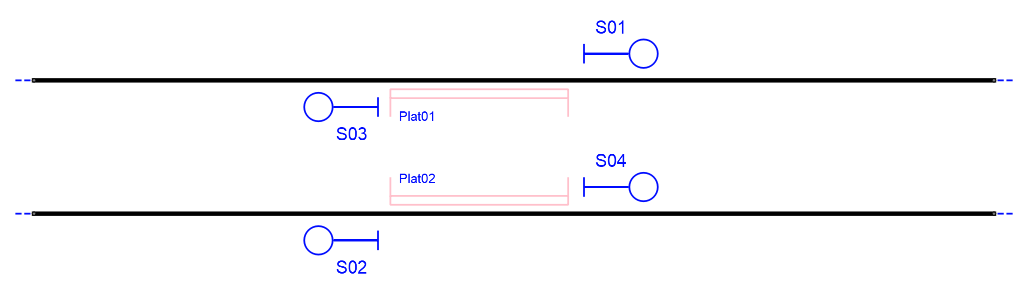
\includegraphics[width=1\textwidth]{Figuras/platforms.PNG}
        \centering\caption{Señalamiento generado para estaciones ferroviarias.}
        \label{fig:signal_platform}
    \end{figure}
    
    Una formación que circule de izquierda a derecha deberá detenerse antes de la señal S01, en caso de utilizar la vía superior, o antes de la señal S04, en caso de utilizar la vía inferior. Análogamente, las formaciones deberán detenerse antes de las señales S03 y S02 en el caso de transitar de derecha a izquierda por la vía superior o inferior respectivamente. Sólo cuando estas señales otorguen a la formación autoridad para circular podrán reanudar su marcha hasta la próxima señal disponible, fuera del alcance de lo ilustrado en la Figura \ref{fig:signal_platform}.
    \subsection{Cruces de via}

\lipsum[1-2]

    \begin{algorithm}[hbt!]
        \caption{Level crossing algorithm}\label{alg:LC}
        \DontPrintSemicolon
        %\SetAlgoLined
        \SetNoFillComment
        \LinesNotNumbered 
        \For { netElement WITH LevelCrossing }
        {
            \tcc{Before reaching level crossing}
            [Signals] $\gets$ ADD circulation signal $>>>$\;
            \tcc{After leaving level crossing}
            [Signals] $\gets$ ADD circulation signal $<<<$\;
        }
        \KwResult{[Signals]} 
    \end{algorithm}

\lipsum[1]
\includegraphics{example-image}\\
\lipsum[1-2]
    \subsection{Maquinas de cambios}
	\label{sec:signal_switches}
	
    % Autoridad > derecho limitado a una porcion
    % Claridad > autoridad no ambigua
    % Anticipacion > avisar con antelacion
    % Granularidad > rutas cortas y funcionales
    % Terminalidad > avisar fin de via
    % Infraestructura > avisar de infraestructura
    % No bloqueo > circulacion fluida
    
    En la Sección \ref{sec:switches} definimos la clase switches que modela a las máquinas de cambios. Las máquinas de cambios son de los elementos ferroviarios mas críticos de la red. Por lo tanto, se deberá aplicar al principio de infraestructura a cada una de sus entradas. Además, las máquinas de cambios actúan como una frontera entre las ramas principales de la red, donde se circula a mayor velocidad, y las ramas secundarias, donde se circula a una velocidad menor. Esto divide las rutas en dos o mas rutas, aplicando el principio de autoridad y granularidad. Finalmente, por el principio de no bloqueo, será necesario generar señales de diferente tipo para las ramas principales y las secundarias, priorizando las primeras. Esto puede cumplirse si otorgamos señales de circulación de tres o mas aspectos a la rama principal y señales de maniobra para utilizar una rama secundaria como salida o entrada de la red.
    
    En el Algoritmo \ref{alg:SW} definimos al punto de acceso de inicio como la vía desde la cual la trayectoria de la formación se bifurca, para lo cual se genera una señal de circulación para continuar por la rama principal y una señal de maniobra para acceder a la rama secundaria. Además, se añade una señal de circulación en la rama principal y una señal de maniobra en la rama secundaria, ambas en sentido contrario, para poder retornar al punto de inicio. 
    
    \begin{algorithm}[hbt!]
        \caption{Algoritmo de generación de señalamiento para Switches}\label{alg:SW}
        \DontPrintSemicolon
        %\SetAlgoLined
        \SetNoFillComment
        \LinesNotNumbered 
        \For { Switch in Switches }
        {
            \tcc{All signals must point to switch}
            \Switch{ Switch.Type }
            {
                \Case{Start}
                {
                    [Signals] $\gets$ ADD circulation signal\;
                    [Signals] $\gets$ ADD maneuver signal\;
                }
                \Case{Continue branch}
                {
                    [Signals] $\gets$ ADD circulation signal\;
                }
                \Case{Detour branch}
                {
                    [Signals] $\gets$ ADD maneuver signal\;
                }
            }   
        }
        \KwResult{[Signals]} 
    \end{algorithm}

    Aplicando el Algoritmo \ref{alg:SW} a un sistema de vías que se bifurcan obtenemos el resultado ilustrado en la Figura \ref{fig:signal_swithces}. Se asumieron que ambas vías son bidireccionales. En caso contrario, si el sentido de circulación es únicamente de bifurcación, las señales de retorno S02 y S03 no son necesarias. Si el sentido de circulación fuese de derecha a izquierda, las señales de inicio S01 no son necesarias.
    
    \begin{figure}[h!]
        \centering
        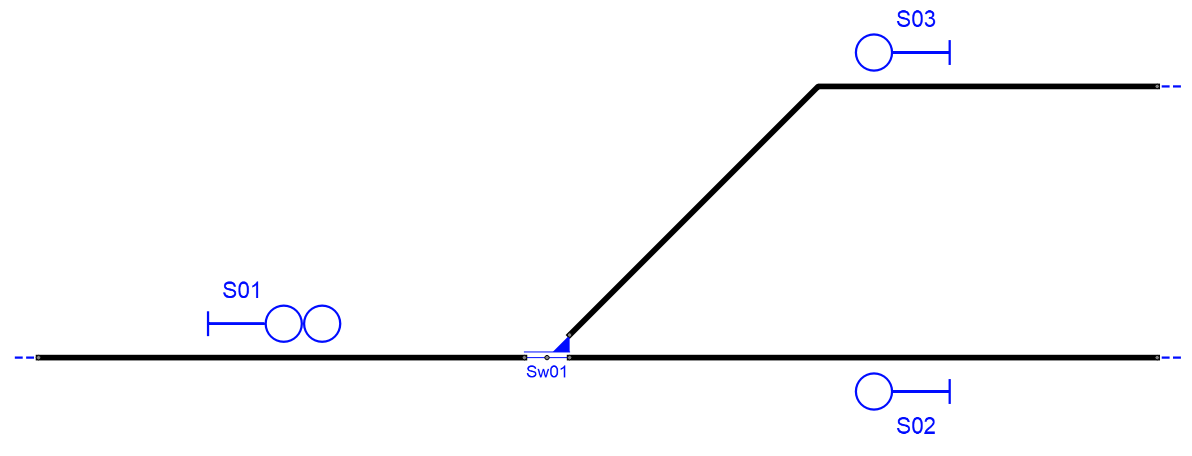
\includegraphics[width=1\textwidth]{Figuras/switches.PNG}
        \centering\caption{Señalamiento generado para cambios de vías.}
        \label{fig:signal_swithces}
    \end{figure}
    
    Una formación que circule de izquierda a derecha deberá detenerse antes de la señal S01. El aspecto mas cercano al poste de la señal S01 indicará si la formación puede circular por la vía principal, como se explicó en la Sección \ref{sec:signals}, previa confirmación por parte del sistema de enclavamiento de que el cambio Sw01 se encuentra en posición normal. De la misma forma, el sistema de enclavamiento confirmará que el cambio Sw01 se encuentra en posición reverso previo a habilitar la circulación por la vía secundaria mediante el aspecto mas alejado al poste de la señal S01.

    Una formación circulando de derecha a izquierda hará uso de las señales S02 y S03 si se encuentran en las vías principal o secundaria respectivamente. Las señales se habilitarán si el sistema de enclavamientos confirma que el cambio Sw01 se encuentra en la posición normal o reverso respectivamente y si no hay formaciones ocupando la vía de inicio donde se encuentra la señal S01, continuando su marcha hasta la próxima señal disponible, fuera del alcance de lo ilustrado en la Figura \ref{fig:signal_swithces}.    